% Capitolo 4

\chapter{Un prototipo di servizio federato}
\label{Capitolo4}
\lhead{Capitolo 4. \emph{Un prototipo di servizio federato}}

L'uso delle tecnologie digitali offre nuove possibilità per
l'educazione. Molte comunità, afferenti alla RM, hanno iniziato la
produzione di materiale pedagogico audio-visuale, che con l'aiuto
della rete, potrebbe contribuire ad arricchire i programmi educativi
pubblici spesso carenti e poco integrati con la cultura quilombola. Il
\emph{Núcleo de Pesquisa e Desenvolvimento Digital (NPDD)}\footnote{Il
  \emph{Núcleo de Pesquisa e Desenvolvimento Digital (NPDD)} della RM
  ricerca e sviluppa tecnologie digitali per la comunicazione, la
  produzione di energie rinnovabili e sostenibili, e il miglioramento
  delle condizioni di vita in simbiosi con l'ambiente. Maggiori
  informazioni su \url{http://wiki.mocambos.net/wiki/NPDD}.}, nucleo
di ricerca e sviluppo digitale della RM, con il progetto \emph{Tambor
  e Comunicação}\footnote{Il progetto \emph{Tambor e Comunicação} é un
  tentativo di fortificare la rete di comunicazione digitale per le
  necessità delle comunità. Vedi
  \url{http://wiki.mocambos.net/wiki/Projeto_Tambor_e_Comunicacao}.},
ha iniziato la ricerca e sviluppo di una soluzione per la
pubblicazione e diffusione in rete di immagini, audio e video di
interesse comune e spesso prodotti nelle stesse comunità.

\section{Sistema di pubblicazione e diffusione di contenuti
  multimediali}
Il sistema prevede l'installazione di un portale sul server locale
delle comunità su cui è possibile pubblicare contenuti multimediali
sfruttando l'alta velocità della rete locale. Il sistema si prende
cura di diffondere i contenuti, etichettati come di interesse comune,
verso i server delle altre comunità. Il prototipo sviluppato cerca di
risolvere le limitazioni di banda della rete rispettando la specifica
di requisiti. 

\section{Archivio multimediale}
L'archivio locale della comunità è un \emph{repository git-annex} che
viene gestito tramite il portale comunitario, sia per la pubblicazione
che per la visualizzazione dei contenuti. L'accesso diretto ai dati è
comunque garantito essendo i dati salvati in chiaro sul disco. 

\subsection{git-annex}
\emph{git-annex} permette la gestione di file con \emph{git}, senza la necessità di
aggiungere il file dentro \emph{git}. Anche se può sembrare paradossale, è
utile quando si ha a che fare con file molto grandi che \emph{git}
attualmente non può gestire facilmente per limitazioni dovute a
memoria, tempo o spazio nel disco.

Anche senza mantenere traccia del contenuto del file, avere la 
possibilità di gestire i file con \emph{git}, di spostarli e cancellarli su un
albero di cartelle versionato, con uso di branches e di cloni
distribuiti, sono tutte buoni motivi per usare \emph{git}. E i file allegati
(da cui il nome \emph{git annex}) possono coesistere nello stesso repository
\emph{git} con i file regolarmente versionati.


\section{Portale Comunitario}
Per lo sviluppo di un portale locale è stato scelto l'uso del
framework \emph{Django}.

\subsection{Django}
\emph{Django} è un framework per lo sviluppo rapido di applicazioni web.


\begin{figure}[htbp]
  \centering
  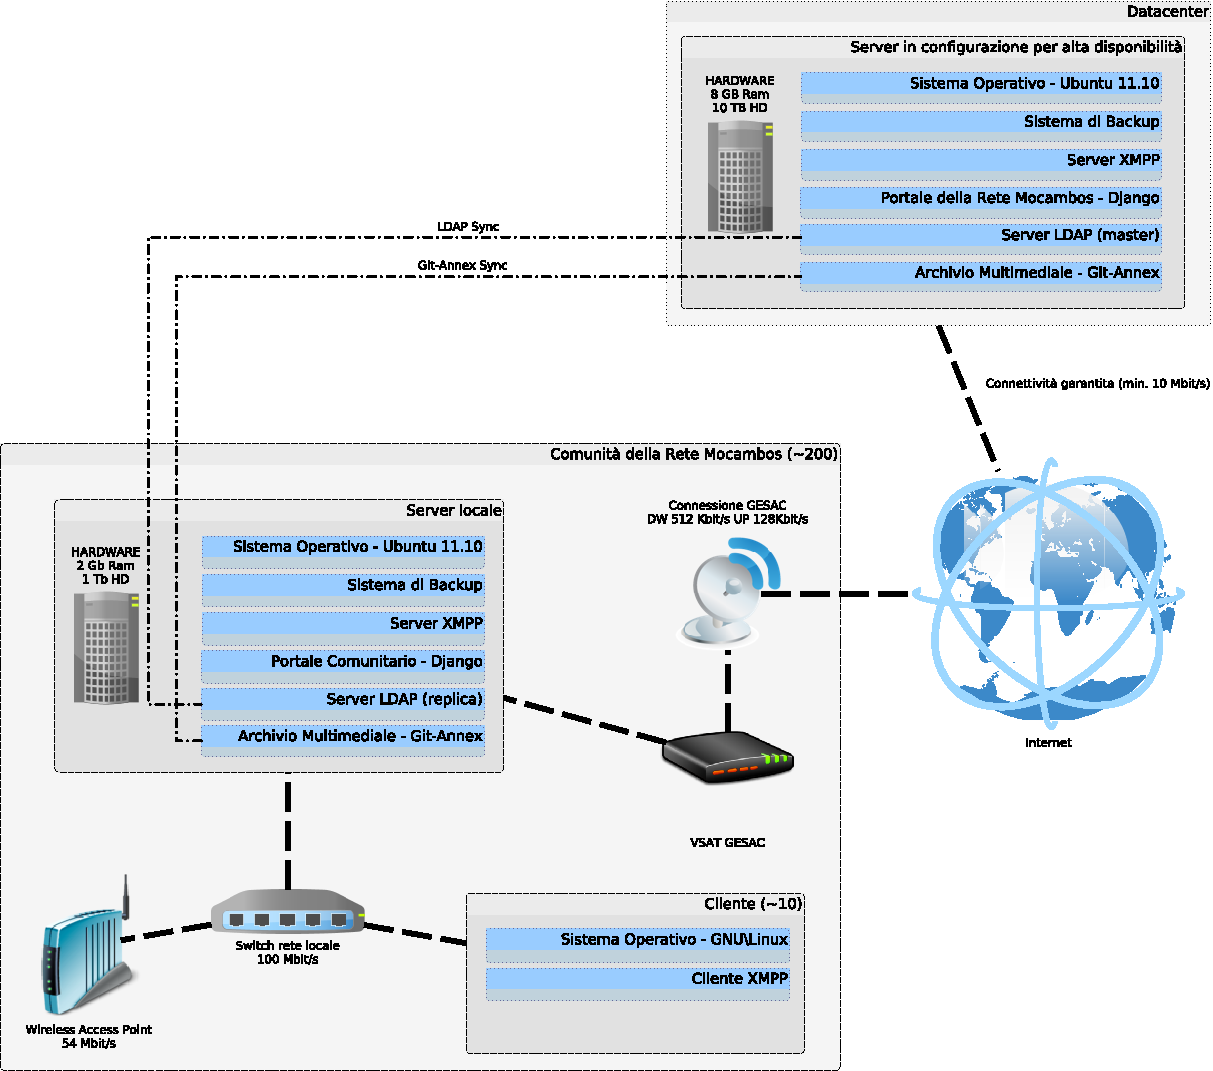
\includegraphics[width=\textwidth]{./Figure/SchemaServer_ReteMocambos-crop.pdf}
  \rule{35em}{0.5pt}
  \caption[Schema dell'infrastruttura della RM]{Schema dell'infrastruttura della RM.}
  \label{fig:SchemaServer_ReteMocambos}
\end{figure}
